\chapter{The Network Subsystem}
\label{chap:networking}

When Andrew Tanenbaum authored the original editions of \textit{Operating Systems: Design and Implementation}, local area networks were an emerging academic curiosity, and the MINIX operating system possessed no built-in TCP/IP networking stack. Today, an operating system devoid of network capabilities is functionally inert. Web browsers, cloud repositories, remote shells, distributed file systems, and automated package managers depend continuously on high-throughput, low-latency, packet-switched networking.

Integrating an enterprise-grade networking stack into a microkernel presents demanding architectural requirements:
\begin{enumerate}
    \item \textbf{Line-Rate Throughput:} At Gigabit and 10-Gigabit speeds, over one million packets can cross the physical wire every second. Copying packet payloads through multiple kernel memory boundaries exhausts memory bus bandwidth and destroys cache locality.
    \item \textbf{Complex Protocol State Machines:} The Transmission Control Protocol (TCP) requires sophisticated sliding window flow control, retransmission timers, congestion control algorithms, and multi-state lifecycle management.
    \item \textbf{POSIX Socket Compatibility:} Modern application workloads (including web browsers like Brave and graphical environments like KDE Plasma) demand complete compatibility with the BSD Socket API and non-blocking event multiplexing via \texttt{epoll}.
\end{enumerate}

In this chapter, we dissect the layered network architecture, examine the physical operation of the Intel 82540EM Gigabit Ethernet controller, explore circular DMA descriptor rings, walk through the protocol pipeline (ARP, IPv4, ICMP, UDP, TCP, and DHCP), and analyze how Hydra powers high-concurrency desktop networking in an isolated Ring~3 driver process.

% ==============================================================================
\section{Layered Network Architectures: The End-to-End Principle}
\label{sec:net_layers}
% ==============================================================================

Computer networks are structured as hierarchies of layers, where each layer provides a well-defined service to the layer above while hiding the implementation details of the layer below.

\subsection{The OSI Model vs. the Internet Protocol Suite}
The theoretical Open Systems Interconnection (OSI) 7-layer model defines Physical, Data Link, Network, Transport, Session, Presentation, and Application layers. In modern operating systems, the pragmatic 4-layer Internet Protocol suite (TCP/IP) is universally adopted:

\begin{figure}[htbp]
\centering
\begin{tikzpicture}[scale=0.9, every node/.style={transform shape}]
    \matrix (stack) [matrix of nodes, nodes={draw=hydrablue, minimum width=10cm, minimum height=0.8cm, fill=white, font=\small\sffamily}, column sep=0mm, row sep=1.5mm] {
        \textbf{Application Layer:} HTTP, HTTPS, DNS, SSH, DHCP, Wayland IPC \\
        \textbf{Transport Layer:} TCP (Streams / Connections) \quad\textbar\quad UDP (Datagrams) \\
        \textbf{Internet Layer:} IPv4 / IPv6 (Routing) \quad\textbar\quad ICMP (Diagnostics) \quad\textbar\quad ARP (MAC Resolution) \\
        \textbf{Link / Physical Layer:} Ethernet (IEEE 802.3) \quad\textbar\quad Intel 82540EM PCIe Controller \\
    };
\end{tikzpicture}
\caption{The Layered Network Protocol Stack.}
\label{fig:net_layers}
\end{figure}

\subsection{Encapsulation and Decapsulation}
When an application transmits data (for example, a browser requesting an HTML page):
\begin{enumerate}
    \item The application deposits the HTTP request string (\texttt{"GET / HTTP/1.1"}) into a socket buffer.
    \item The \textbf{Transport Layer (TCP)} prepends a 20-byte TCP header containing source/destination port numbers, sequence numbers, and control flags, forming a \textbf{TCP Segment}.
    \item The \textbf{Internet Layer (IPv4)} prepends a 20-byte IPv4 header containing source/destination IP addresses, Time-to-Live (TTL), and protocol identifiers, forming an \textbf{IP Packet}.
    \item The \textbf{Link Layer (Ethernet)} prepends a 14-byte Ethernet header (Destination MAC, Source MAC, EtherType) and appends a 4-byte Cyclic Redundancy Check (CRC32), forming an \textbf{Ethernet Frame}.
    \item The physical network interface card (NIC) serializes the frame into electrical signals onto the wire.
\end{enumerate}

Upon arrival at the destination machine, the hardware and driver perform the reverse operation: stripping headers, verifying checksums, and delivering the raw payload to the listening user socket.

% ==============================================================================
\section{The Intel 82540EM (e1000) Network Controller}
\label{sec:e1000_hardware}
% ==============================================================================

Hydra targets the industry-standard **Intel 82540EM Gigabit Ethernet Controller**, supported natively on physical hardware and standard virtual machine hypervisors (VirtualBox, QEMU, VMware).

The e1000 controller connects to the processor via the PCI / PCI Express bus. It acts as an autonomous bus-master device capable of streaming data directly to and from physical RAM without CPU intervention.

\subsection{PCI Discovery and MMIO Register Aperture}
During boot, Hydra's PCI scanner enumerates the configuration space, matching Vendor ID \texttt{0x8086} (Intel) and Device ID \texttt{0x100E} (82540EM). The kernel reads Base Address Register 0 (\texttt{BAR0}), which specifies the physical base address of the controller's 128~KiB Memory-Mapped I/O (MMIO) register aperture.

Key controller registers include:
\begin{itemize}
    \item \textbf{\texttt{CTRL} (Offset \texttt{0x0000}):} Device Control register. Software writes bit 26 (\texttt{RST}) to perform a hardware master reset, and configures speed (1000 Mbps Full Duplex) and auto-negotiation.
    \item \textbf{\texttt{STATUS} (Offset \texttt{0x0008}):} Device Status register. Indicates link state (UP/DOWN) and transmission duplex.
    \item \textbf{\texttt{RCTL} (Offset \texttt{0x0100}):} Receive Control register. Enables the receiver (\texttt{EN}), configures receive buffer size (e.g., 2048 bytes), and strips Ethernet CRC.
    \item \textbf{\texttt{TCTL} (Offset \texttt{0x0400}):} Transmit Control register. Enables transmission (\texttt{EN}) and collision detection parameters.
    \item \textbf{\texttt{RAL} / \texttt{RAH} (Offset \texttt{0x5400}):} Receive Address Low and High registers. Stores the 48-bit physical Ethernet MAC address harvested from the card's non-volatile EEPROM.
\end{itemize}

% ==============================================================================
\section{Circular DMA Descriptor Rings}
\label{sec:dma_descriptor_rings}
% ==============================================================================

To sustain high-speed packet processing without interrupting the CPU on every individual frame, the e1000 utilizes circular **DMA Descriptor Rings** in physical memory:

\begin{figure}[htbp]
\centering
\begin{tikzpicture}[scale=0.88, every node/.style={transform shape}]
    % Circular ring represented as linked boxes
    \def\radius{2.8cm}
    \foreach \i in {0,...,7} {
        \node[draw=hydrablue, fill=white, rounded corners, minimum size=1.1cm] (desc\i) at ({-\i*45 + 90}:\radius) {\footnotesize \texttt{Desc \i}};
    }
    
    % Center label
    \node[align=center, font=\sffamily\bfseries\color{hydrablue}] at (0,0) {Circular Rx Ring\\ \footnotesize 128 Descriptors};

    % Arrows connecting circular ring
    \draw[->, >=Stealth, line width=1.2pt, hydragray] (desc0) to[bend left=20] (desc1);
    \draw[->, >=Stealth, line width=1.2pt, hydragray] (desc1) to[bend left=20] (desc2);
    \draw[->, >=Stealth, line width=1.2pt, hydragray] (desc2) to[bend left=20] (desc3);
    \draw[->, >=Stealth, line width=1.2pt, hydragray] (desc3) to[bend left=20] (desc4);
    \draw[->, >=Stealth, line width=1.2pt, hydragray] (desc4) to[bend left=20] (desc5);
    \draw[->, >=Stealth, line width=1.2pt, hydragray] (desc5) to[bend left=20] (desc6);
    \draw[->, >=Stealth, line width=1.2pt, hydragray] (desc6) to[bend left=20] (desc7);
    \draw[->, >=Stealth, line width=1.2pt, hydragray] (desc7) to[bend left=20] (desc0);

    % Pointers
    \node[above=0.3cm of desc0, font=\bfseries\footnotesize\color{rustred}] {Head (Hardware writes here)};
    \node[right=0.3cm of desc2, font=\bfseries\footnotesize\color{rustkeyword}] {Tail (Driver reaps here)};
\end{tikzpicture}
\caption{Circular DMA Descriptor Ring Architecture of the Intel E1000 Controller.}
\label{fig:e1000_ring}
\end{figure}

\subsection{The Receive (Rx) Descriptor Structure}
Hydra pre-allocates a circular array of 128 Receive Descriptors in non-swappable physical memory. Each descriptor is 16 bytes:

\begin{lstlisting}[language=Rust, caption={Intel E1000 Receive Descriptor (\texttt{src/net/e1000.rs})}]
#[repr(C)]
pub struct RxDescriptor {
    pub buffer_addr: u64, // Physical address of 2048-byte receive buffer
    pub length: u16,      // Length of received packet in bytes
    pub checksum: u16,    // Hardware-computed packet checksum
    pub status: u8,       // Descriptor status (Descriptor Done DD, End of Packet EOP)
    pub errors: u8,       // Hardware error flags (CRC error, symbol error)
    pub special: u16,     // VLAN tag
}
\end{lstlisting}

When an Ethernet frame arrives from the network:
\begin{enumerate}
    \item The card's DMA engine reads the descriptor pointed to by its internal \texttt{RDH} (Receive Descriptor Head) register.
    \item The hardware streams the packet bytes across the PCI bus directly into \texttt{buffer\_addr} in physical RAM.
    \item The hardware sets the \texttt{status} byte to indicate Descriptor Done (\texttt{DD}) and End-of-Packet (\texttt{EOP}), sets \texttt{length}, and increments the \texttt{RDH} pointer.
    \item The hardware asserts IRQ~11.
    \item Hydra's Ring~3 driver processes the packet from the buffer pointed to by \texttt{RDT} (Receive Descriptor Tail), resets the descriptor status, and advances \texttt{RDT}.
\end{enumerate}

Because packets are streamed directly into physical RAM mapped into the driver process, \textbf{zero memory copies are performed in the microkernel}!

% ==============================================================================
\section{The Network Protocol Pipeline}
\label{sec:protocol_pipeline_deep}
% ==============================================================================

Once a packet is harvested from the Rx descriptor ring, it enters Hydra's layered protocol pipeline (\texttt{src/net/stack.rs}):

\subsection{Ethernet Framing and the Address Resolution Protocol (ARP)}
At the link layer, packets are addressed via 48-bit Media Access Control (MAC) addresses (e.g., \texttt{08:00:27:41:47:51}). However, internet applications communicate using 32-bit IPv4 addresses (e.g., \texttt{10.0.2.15}).

The **Address Resolution Protocol (ARP)** maps IP addresses to physical MAC addresses:
\begin{itemize}
    \item When transmitting to an IP address on the local subnet whose MAC address is unknown, Hydra broadcasts an **ARP Request** frame to the broadcast MAC (\texttt{FF:FF:FF:FF:FF:FF}): \textit{"Who has 10.0.2.2? Tell 10.0.2.15"}.
    \item The target gateway node replies with an **ARP Reply** unicast packet: \textit{"10.0.2.2 is at 52:54:00:12:35:02"}.
    \item Hydra stores this mapping in its high-speed in-memory **ARP Cache**, with automatic timestamp expiration.
\end{itemize}

\subsection{The Internet Protocol (IPv4) and ICMP}
The IPv4 layer inspects incoming frames whose EtherType is \texttt{0x0800}:
\begin{enumerate}
    \item \textbf{Header Validation:} Verifies that the version is 4, header length is $\ge 20$ bytes, and the 16-bit Internet Header Checksum is mathematically valid.
    \item \textbf{Destination Verification:} Verifies that the destination IP matches the host's assigned IP (\texttt{10.0.2.15}) or the subnet broadcast address.
    \item \textbf{Protocol Demultiplexing:} Inspects the \texttt{protocol} byte:
    \begin{itemize}
        \item \texttt{0x01} (ICMP): Internet Control Message Protocol. Handles diagnostic \texttt{ECHO\_REQUEST} (ping) packets by immediately formulating an \texttt{ECHO\_REPLY} and returning it to the sender.
        \item \texttt{0x06} (TCP): Passes the payload to the Transmission Control Protocol engine.
        \item \texttt{0x11} (UDP): Passes the payload to the User Datagram Protocol engine.
    \end{itemize}
\end{enumerate}

\subsection{The User Datagram Protocol (UDP) and DNS Resolution}
UDP is a connectionless, lightweight transport protocol. Each UDP datagram contains an 8-byte header specifying Source Port, Destination Port, Length, and Checksum.

In Hydra, UDP powers domain name resolution:
\begin{itemize}
    \item When a user types a URL (e.g., \texttt{msn.com} or \texttt{google.com}) into the Brave web browser, the browser issues a standard DNS query to the nameserver (\texttt{10.0.2.3}) on UDP Port 53.
    \item Hydra transmits the datagram, records the query transaction ID, and suspends the calling thread on a socket wait queue.
    \item When the DNS response packet arrives over the wire, Hydra's socket demultiplexer matches the port, extracts the IP address record, and immediately awakens the browser thread.
\end{itemize}

\subsection{The Transmission Control Protocol (TCP) State Machine}
TCP provides a reliable, connection-oriented, full-duplex byte stream. It guarantees that bytes are delivered in order, without duplicates or loss, despite an unreliable underlying packet-switched network.

Hydra's TCP implementation (\texttt{src/net/tcp.rs}) tracks the standardized TCP state machine:
\begin{enumerate}
    \item \textbf{Three-Way Handshake (Connection Establishment):}
    \begin{equation}
        \text{Client} \xrightarrow{\quad\text{SYN}\quad} \text{Server} \xrightarrow{\quad\text{SYN-ACK}\quad} \text{Client} \xrightarrow{\quad\text{ACK}\quad} \text{Server}
    \end{equation}
    \item \textbf{Sliding Window Flow Control:} Senders maintain sequence numbers and window sizes advertised by the receiver, ensuring that the sender never transmits more bytes than the receiver's socket buffer can accommodate.
    \item \textbf{Four-Way Handshake (Connection Teardown):} Either party initiates closure by transmitting a segment with the \texttt{FIN} flag set, followed by mutual acknowledgements and entry into the \texttt{TIME\_WAIT} state to ensure lingering duplicate packets expire.
\end{enumerate}

% ==============================================================================
\section{Automatic Network Configuration via DHCP}
\label{sec:dhcp_deep}
% ==============================================================================

In modern networking, manually configuring static IP addresses, subnet masks, and DNS servers is unacceptable. Hydra implements an automated **Dynamic Host Configuration Protocol (DHCP)** client:

\begin{figure}[htbp]
\centering
\begin{tikzpicture}[scale=0.88, every node/.style={transform shape}]
    \node[draw=rustkeyword, fill=white, rounded corners, minimum width=3cm, minimum height=1cm] (client) at (0, 4) {\textbf{Hydra Client}};
    \node[draw=hydrablue, fill=white, rounded corners, minimum width=3cm, minimum height=1cm] (server) at (8, 4) {\textbf{DHCP Server}};

    \draw[->, >=Stealth, line width=1.2pt] (0, 3.2) -- node[above] {\small 1. \texttt{DHCPDISCOVER} (Broadcast)} (8, 2.6);
    \draw[<-, >=Stealth, line width=1.2pt] (0, 2.0) -- node[above] {\small 2. \texttt{DHCPOFFER} (Unicast \texttt{10.0.2.15})} (8, 1.4);
    \draw[->, >=Stealth, line width=1.2pt] (0, 0.8) -- node[above] {\small 3. \texttt{DHCPREQUEST} (Request lease)} (8, 0.2);
    \draw[<-, >=Stealth, line width=1.2pt] (0, -0.4) -- node[above] {\small 4. \texttt{DHCPACK} (Commit Gateway, DNS, Mask)} (8, -1.0);
\end{tikzpicture}
\caption{The DHCP Four-Step DORA Protocol Exchange.}
\label{fig:dhcp_dora}
\end{figure}

During boot, Hydra's network daemon broadcasts a \texttt{DHCPDISCOVER} packet on UDP Port 67. The DHCP server responds with \texttt{DHCPOFFER}, assigning:
\begin{itemize}
    \item Assigned IP Address: \texttt{10.0.2.15}
    \item Default Gateway: \texttt{10.0.2.2}
    \item Subnet Mask: \texttt{255.255.255.0}
    \item Domain Name Server: \texttt{10.0.2.3}
\end{itemize}
Hydra commits these values to its internal routing table and automatically populates the POSIX \texttt{/etc/resolv.conf} virtual file, ensuring that graphical applications immediately have working internet access upon boot.

% ==============================================================================
\section{Socket Polling and High-Concurrency Event Multiplexing}
\label{sec:epoll_deep}
% ==============================================================================

High-performance applications (such as the Brave web browser, Python asynchronous servers, and desktop compositors) manage hundreds of concurrent network connections simultaneously.

\subsection{The Inefficiency of \texttt{select()} and \texttt{poll()}}
Historically, UNIX systems utilized \texttt{select()} and \texttt{poll()}:
\begin{itemize}
    \item An application passed an array of 1,000 file descriptors to the kernel on every single iteration of its event loop.
    \item The kernel performed an $O(N)$ linear scan across all 1,000 descriptors to check for readable data.
    \item As concurrency grew, CPU utilization skyrocketed simply scanning idle sockets.
\end{itemize}

\subsection{The Linux \texttt{epoll} Architecture in Hydra}
To achieve true $O(1)$ scalability, Hydra implements complete Linux-compatible **\texttt{epoll(7)}** semantics in \texttt{src/compat/linux/epoll.rs}:
\begin{enumerate}
    \item \textbf{\texttt{epoll\_create1()}:} Allocates an epoll state object holding an in-kernel Red-Black tree and a Ready List.
    \item \textbf{\texttt{epoll\_ctl()}:} Adds, modifies, or deletes monitored file descriptors. The socket registers an internal task waker with its wait queue.
    \item \textbf{\texttt{epoll\_wait()}:} The application thread sleeps. When a packet arrives over the network, the hardware interrupt wakes the driver, which deposits data into the socket buffer and appends the socket to the epoll Ready List in $O(1)$ time. The application awakens immediately with the exact list of active descriptors!
\end{enumerate}

% ==============================================================================
\section{Domain Name System (DNS) Resolution and Wire Protocols}
\label{sec:dns_deep}
% ==============================================================================

While the transport layer routes datagrams using 32-bit numerical IPv4 addresses (such as \texttt{142.250.190.46}), human users and graphical web browsers address network resources via domain names (e.g., \texttt{google.com} or \texttt{msn.com}).

Hydra implements an RFC~1035 compliant Domain Name System (DNS) resolver directly within \texttt{src/net/dns.rs}. The client translates hostnames into 32-bit IPv4 addresses over User Datagram Protocol (UDP) destination port 53.

\subsection{RFC 1035 Packet Layout and Label Encoding}

DNS messages follow a strict binary wire format divided into header, question, answer, authority, and additional record sections:

\begin{figure}[htbp]
\centering
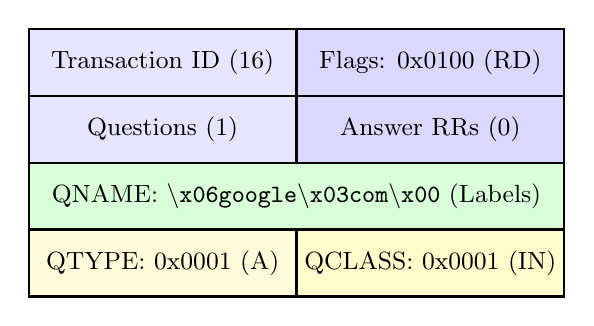
\begin{tikzpicture}[scale=0.85]
    \draw[thick, fill=blue!10] (0, 3) rectangle (4, 4) node[pos=.5] {\small Transaction ID (16)};
    \draw[thick, fill=blue!15] (4, 3) rectangle (8, 4) node[pos=.5] {\small Flags: 0x0100 (RD)};
    \draw[thick, fill=blue!10] (0, 2) rectangle (4, 3) node[pos=.5] {\small Questions (1)};
    \draw[thick, fill=blue!15] (4, 2) rectangle (8, 3) node[pos=.5] {\small Answer RRs (0)};
    \draw[thick, fill=green!15] (0, 1) rectangle (8, 2) node[pos=.5] {\small QNAME: \texttt{\textbackslash x06google\textbackslash x03com\textbackslash x00} (Labels)};
    \draw[thick, fill=yellow!15] (0, 0) rectangle (4, 1) node[pos=.5] {\small QTYPE: 0x0001 (A)};
    \draw[thick, fill=yellow!20] (4, 0) rectangle (8, 1) node[pos=.5] {\small QCLASS: 0x0001 (IN)};
\end{tikzpicture}
\caption{RFC 1035 DNS Query Message Binary Layout.}
\label{fig:dns_wire_format}
\end{figure}

Domain names are encoded as sequences of length-prefixed labels. The string \texttt{"google.com"} is encoded as:
\begin{equation}
\text{Wire Format} = [6, \text{'g'}, \text{'o'}, \text{'o'}, \text{'g'}, \text{'l'}, \text{'e'}, 3, \text{'c'}, \text{'o'}, \text{'m'}, 0]
\end{equation}
The trailing null byte (\texttt{0x00}) signals the root domain.

\begin{lstlisting}[language=Rust, caption={DNS Query Construction and Answer Parsing (\texttt{src/net/dns.rs})}]
pub const DNS_PORT: u16        = 53;
pub const DNS_CLIENT_PORT: u16 = 53535;

/// Serializes an RFC 1035 recursive A-record query packet.
pub fn build_dns_query(domain: &str, tx_id: u16) -> alloc::vec::Vec<u8> {
    let mut packet = alloc::vec::Vec::with_capacity(64);

    // 1. Transaction ID & Standard Query Flags (RD = 1: Recursion Desired)
    packet.extend_from_slice(&tx_id.to_be_bytes());
    packet.extend_from_slice(&0x0100u16.to_be_bytes()); // Flags
    packet.extend_from_slice(&1u16.to_be_bytes());      // 1 Question
    packet.extend_from_slice(&0u16.to_be_bytes());      // 0 Answers
    packet.extend_from_slice(&0u16.to_be_bytes());      // 0 Authority
    packet.extend_from_slice(&0u16.to_be_bytes());      // 0 Additional

    // 2. Encode QNAME as length-prefixed labels
    for part in domain.split('.') {
        if part.is_empty() { continue; }
        packet.push(part.len() as u8);
        packet.extend_from_slice(part.as_bytes());
    }
    packet.push(0); // Zero-length label for root domain

    // 3. QTYPE (0x0001 = Type A, IPv4) & QCLASS (0x0001 = Internet IN)
    packet.extend_from_slice(&1u16.to_be_bytes());
    packet.extend_from_slice(&1u16.to_be_bytes());

    packet
}

/// Parses an RFC 1035 DNS answer section and extracts the first IPv4 address.
pub fn parse_dns_response(buf: &[u8], tx_id: u16) -> Option<[u8; 4]> {
    if buf.len() < 12 { return None; }

    let resp_id = u16::from_be_bytes([buf[0], buf[1]]);
    if resp_id != tx_id { return None; } // ID mismatch

    let answers = u16::from_be_bytes([buf[6], buf[7]]);
    if answers == 0 { return None; }

    // Skip question section...
    let mut idx = 12;
    while idx < buf.len() && buf[idx] != 0 {
        idx += (buf[idx] as usize) + 1;
    }
    idx += 5; // Skip trailing 0x00, QTYPE (2B), QCLASS (2B)

    // Parse Answer Section: Skip name pointer, Type, Class, TTL
    while idx + 10 <= buf.len() {
        let type_code = u16::from_be_bytes([buf[idx + 2], buf[idx + 3]]);
        let data_len = u16::from_be_bytes([buf[idx + 8], buf[idx + 9]]) as usize;
        idx += 10;

        if type_code == 1 && data_len == 4 && idx + 4 <= buf.len() {
            // Found Type A IPv4 address!
            return Some([buf[idx], buf[idx + 1], buf[idx + 2], buf[idx + 3]]);
        }
        idx += data_len;
    }

    None
}
\end{lstlisting}

\subsection{DNS Troubleshooting in Complex Browser Workloads}
When running full modern desktop web browsers (such as Brave), DNS failures typically manifest as \texttt{DNS\_PROBE\_POSSIBLE} or \texttt{ERR\_NAME\_NOT\_RESOLVED}. In a microkernel architecture, diagnosing these issues requires verifying:
\begin{enumerate}
    \item \textbf{DHCP Option 6 Propagation:} That the DHCP client correctly extracted the DNS server address (e.g., \texttt{10.0.2.3} under QEMU or VirtualBox NAT) and updated \texttt{/etc/resolv.conf}.
    \item \textbf{Ephemeral UDP Port Binding:} That outbound packets with source port \texttt{53535} are correctly translated by the hypervisor NAT table.
    \item \textbf{Transaction ID Matching:} That delayed or out-of-order UDP response datagrams do not cause premature lookup aborts.
\end{enumerate}

% ==============================================================================
\section{Summary}
\label{sec:summary_chap6}
% ==============================================================================

Modern operating systems require high-performance, fault-isolated networking. Hydra achieves this by running its network stack entirely in an isolated Ring~3 driver process:
\begin{itemize}
    \item Hardware communication with the Intel 82540EM Gigabit NIC is performed via circular DMA descriptor rings, streaming packets directly into physical RAM with zero microkernel copies.
    \item The protocol pipeline cleanly encapsulates ARP resolution, IPv4 routing, ICMP diagnostics, UDP datagrams, and full TCP state machines.
    \item Automated DHCP negotiation establishes dynamic network identity, gateway routing, and DNS configuration on boot.
    \item Linux-compatible \texttt{epoll} event multiplexing delivers scalable, non-blocking I/O for modern web browsers and desktop applications.
\end{itemize}

% ==============================================================================
\section{Exercises and Review Problems}
\label{sec:exercises_chap6}
% ==============================================================================

\begin{enumerate}
    \item \textbf{Encapsulation Overhead:} Calculate the total byte overhead added to an application payload by the Ethernet, IPv4, and TCP headers (assuming no optional header fields). What percentage of a maximum transmission unit (MTU of 1500 bytes) is consumed by headers?
    \item \textbf{DMA Ring Operation:} Explain how the Intel E1000 controller uses Head and Tail pointers in its circular receive descriptor ring. Under what condition does the network card drop incoming packets due to buffer overrun?
    \item \textbf{ARP Mechanics:} Why is ARP necessary if computers already possess IP addresses? What vulnerability arises from the fact that ARP requests and replies are unauthenticated?
    \item \textbf{IP Checksum Verification:} The IPv4 header checksum algorithm uses the 16-bit one's complement sum. Why does the header checksum change at every intermediate router along a packet's journey across the Internet?
    \item \textbf{TCP Three-Way Handshake:} Diagram the three-way handshake used to establish a TCP connection. Why is a two-way handshake insufficient to guarantee mutual agreement on initial sequence numbers?
    \item \textbf{Flow Control vs. Congestion Control:} Distinguish between TCP sliding window flow control and TCP congestion control. Which mechanism protects the receiving host, and which protects the intermediate network routers?
    \item \textbf{TIME\_WAIT State:} Why must a TCP endpoint remain in the \texttt{TIME\_WAIT} state for two Maximum Segment Lifetimes ($2 \times \text{MSL}$) after closing a connection?
    \item \textbf{DHCP DORA Sequence:} Detail the four packets exchanged during a DHCP lease negotiation. Why are the initial discover and request packets sent to the IP broadcast address \texttt{255.255.255.255}?
    \item \textbf{Epoll Scalability:} Why does Linux \texttt{epoll} scale to tens of thousands of connections with $O(1)$ overhead, whereas classic \texttt{select} degrades with $O(N)$ performance?
    \item \textbf{Design Problem:} Design a zero-copy packet transmission pipeline where an application transmits video data from an OpenZFS file directly out of the Intel e1000 network card. How can memory pages be shared across the VFS, file system server, and network driver without allocating intermediate kernel buffers?
\end{enumerate}
